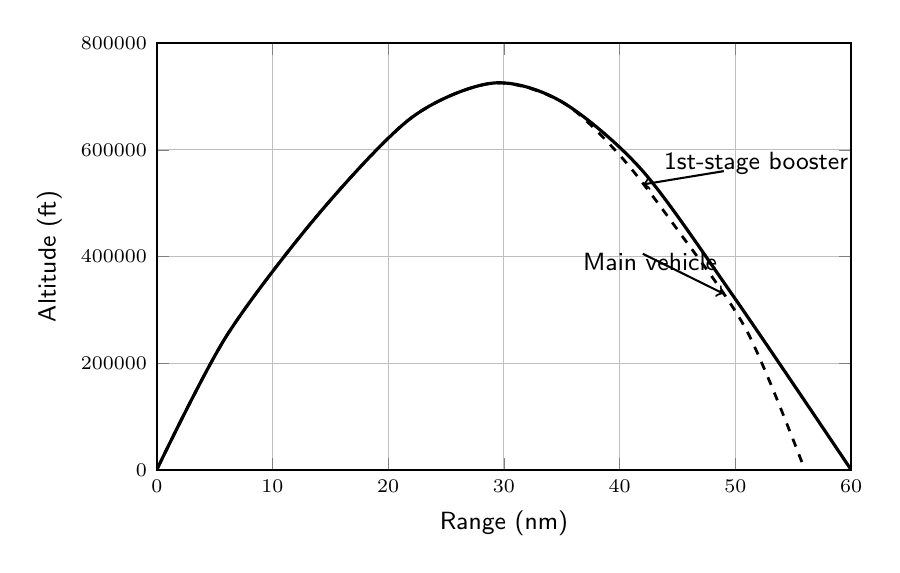
\begin{tikzpicture}
\begin{axis}[
  width=10.4cm,height=7.0cm,
  xmin=0,xmax=60,ymin=0,ymax=800000,
  xtick={0,10,20,30,40,50,60},
  ytick={0,200000,400000,600000,800000},
  grid=major,
  axis line style={line width=0.8pt},
  tick label style={font=\scriptsize},
  label style={font=\sffamily\small},
  xlabel={Range (nm)},ylabel={Altitude (ft)},
  scaled y ticks=false,
  yticklabel style={/pgf/number format/fixed,/pgf/number format/1000 sep={}},
]
  \addplot[line width=1.15pt,smooth] coordinates {(0,0) (6,250000) (14,480000) (22,660000) (29,725000) (35,690000) (42,560000) (50,320000) (60,0)};
  \addplot[line width=1.0pt,dashed,smooth] coordinates {(0,0) (6,250000) (14,480000) (22,660000) (29,725000) (35,690000) (40,590000) (45,450000) (51,260000) (56,0)};
  \node[font=\sffamily\small,anchor=west] at (axis cs:43,575000) {1st-stage booster};
  \draw[->,line width=0.75pt] (axis cs:49,560000)--(axis cs:42,535000);
  \node[font=\sffamily\small,anchor=west] at (axis cs:36,390000) {Main vehicle};
  \draw[->,line width=0.75pt] (axis cs:42,405000)--(axis cs:49,330000);
\end{axis}
\end{tikzpicture}
